\begin{center}
    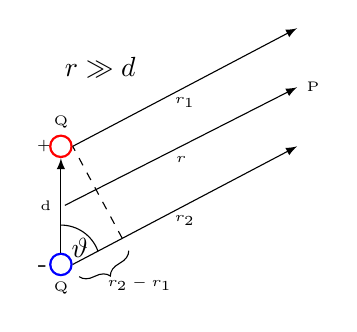
\begin{tikzpicture}
        %Kreise
        \fill[blue]   (0,0) circle (0.15);    %äußerer Kreis
        \fill[white]  (0,0) circle (0.12);     %innerer Kreis
        \node at(-0.05,-0.03)[left]{-};           
        \node at(0,-0.1)[below]{\tiny{Q}}; 

        \node at(0,1.5)[left]{\tiny{+}};
        \fill[red]    (0,1.5) circle (0.15);  %äußerer Kreis
        \fill[white]  (0,1.5) circle (0.12);  %innerer Kreis 
        \node at(0,1.6)[above]{\tiny{Q}};                

        %Pfeile
        \draw[-latex] (0,0.15) -- (0,1.35)
            node[left, midway]{\tiny{d}};
        \draw[-latex] (0.15,1.5) -- (3,3)    
            node[midway, below]{\tiny{$r_1$}};
        \draw[-latex] (0.05,0.75) -- (3,2.25) 
            node[right]{\tiny{P}} 
            node[midway, below]{\tiny{$r$}};
        \draw[-latex] (0.15,0) -- (3,1.5)  
            node[midway, below]{\tiny{$r_2$}};

        %gestrichelte Linie
        \draw[dashed](0.78,0.33) -- (0.15,1.5);

        %Winkel
        \draw[-] (90:0.5) arc (90:20:0.5)
            node[left, yshift=1] {$\vartheta$};

        %Klammer
        \draw [black,
            decorate,
            decoration = {brace,
                    raise=5pt,
                    amplitude=5pt}] (0.78,0.33) -- (0.15,0);
        \node at (1,-0.25) []{\tiny{$r_2-r_1$}};
        %Legende
        \node at(0.5,2.5){$r\gg d$};

    \end{tikzpicture}
\end{center}
